\documentclass[10pt,conference]{IEEEtran}

\usepackage{graphicx}
\usepackage{subcaption}
\usepackage{booktabs}
\usepackage{array}
\usepackage{url}
\usepackage{hyperref}
\usepackage{balance}

\newcommand{\synapse}{Synapse-Works }

\title{Synapse-Works: A Web-Based Visual Framework for Democratizing Neural Network Development}

\author{
    \IEEEauthorblockN{Dhanya V\IEEEauthorrefmark{1}, Suriyaa MM\IEEEauthorrefmark{1}}
    \IEEEauthorblockA{\IEEEauthorrefmark{1}Indian Institute of Technology Tirupati\\
        Tirupati, India\\
        Email: \{dhanya.v, suriyaa.mm\}@iittp.ac.in}
}

\begin{document}

\maketitle

\begin{abstract}
    Despite the rapid growth of machine learning, technical barriers to neural network development remain high for practitioners without strong programming backgrounds. We present \synapse, a web-based visual framework that enables users to design, train, and evaluate neural networks without writing code. Our tool addresses a significant portion of ML debugging challenges that remain unresolved in literature, providing an accessible platform for researchers, educators, and domain experts. Through comprehensive evaluation across multiple neural network architectures (Linear Classification, CNN, U-Net, Segmentation), we demonstrate significant improvements in development time while maintaining computational performance equivalent to manual PyTorch implementations.

    \textbf{Tool Demo Video:} [YouTube URL to be added]\\
    \textbf{Source Code:} \url{https://github.com/SuriyaaMM/synapse-works}
\end{abstract}

\section{Introduction}
The complexity of neural network development creates significant barriers for
domain experts who understand problems that machine learning can solve but lack
technical implementation expertise. Traditional development requires Python
proficiency, CUDA configuration knowledge, and familiarity with multiple
frameworks—skills that many researchers in neuroscience and life sciences lack
formal training
in~\cite{undergrad_quant_neuro_2015}~\cite{python_in_quant_neuro_2015}.

\textbf{Current Challenges:}
\begin{itemize}
    \item Only 48\% of identified ML debugging challenges have been explicitly addressed
          by research, with 46.9\% remaining unresolved or unmentioned. In real-world
          practice, 52.6\% of issues reported on GitHub and 70.3\% of problems discussed
          in practitioner interviews are not addressed by current
          research~\cite{nguyen2025systematicsurveydebuggingtechniques}.
    \item Common errors include dimension mismatches leading to "catastrophic failures"
          during model training or inference, missing validation sets, wrong performance
          metrics, and incorrect train/test data
          splits~\cite{nguyen2025systematicsurveydebuggingtechniques}.
    \item 94\% of enterprises consider AI skills critical, but only one-third feel prepared~\cite{IDC2025AISkillsGap}.
\end{itemize}

We present \synapse, the first comprehensive open-source visual neural network
builder that bridges the gap between educational tools (e.g., TensorFlow
Playground~\cite{tensorflow_playground}) and production frameworks
pytorch~\cite{DBLP:journals/corr/abs-1912-01703}. Our tool enables rapid
prototyping without sacrificing model complexity, supporting architectures from
simple linear models to complex segmentation networks.

\textbf{Contributions:}
\begin{itemize}
    \item A web-based visual framework reducing neural network development barriers by
          significantly decreasing model creation time. Integration of a PyTorch backend
          with advanced visualization through an intuitive node-based user interface.
          Comprehensive evaluation across diverse architectures (Linear, CNN, U-Net,
          Segmentation) demonstrating maintained performance equivalent to standalone
          model scripts. An open-source platform enabling broader community participation
          in deep learning.
\end{itemize}

\section{Related Work and Positioning}
\textbf{Visual ML Tools:} TensorFlow Playground~\cite{tensorflow_playground} provides educational visualization but is limited to simple feedforward networks and toy datasets. Commercial platforms like IBM Watson Studio offer visual interfaces but often have significant cost barriers and vendor lock-in.

\textbf{Traditional ML Tools:} Weka~\cite{hall2009weka}, Orange~\cite{demsar2013orange}, and KNIME~\cite{berthold2007knime}~\cite{berthold2009knime2}excel at data preprocessing and traditional ML but lack comprehensive neural network architecture design capabilities.

\textbf{Academic Tools:} Various research prototypes focus on specific aspects of ML visualization~\cite{hohman2019summit} but often lack comprehensive development environments for real-world applications.

\textbf{Gap Analysis:} No existing tool provides the combination of:
\begin{itemize}
    \item Visual neural network architecture design
    \item Support for complex models (e.g., U-Net, segmentation networks)
    \item Production-ready training capabilities with GPU acceleration
    \item Open-source accessibility
\end{itemize}
\synapse aims to fill this gap by providing comprehensive visual neural network development capabilities that scale from educational use to research and production applications.

\section{System Architecture}
\subsection{Design Philosophy}
\synapse adopts a decoupled client-server architecture optimized for both usability and computational efficiency. The system separates the user interface from compute-intensive operations, enabling the frontend to run on any device while offloading neural network training to specialized hardware like GPUs or TPUs.
\begin{figure}[htbp]
    \centering
    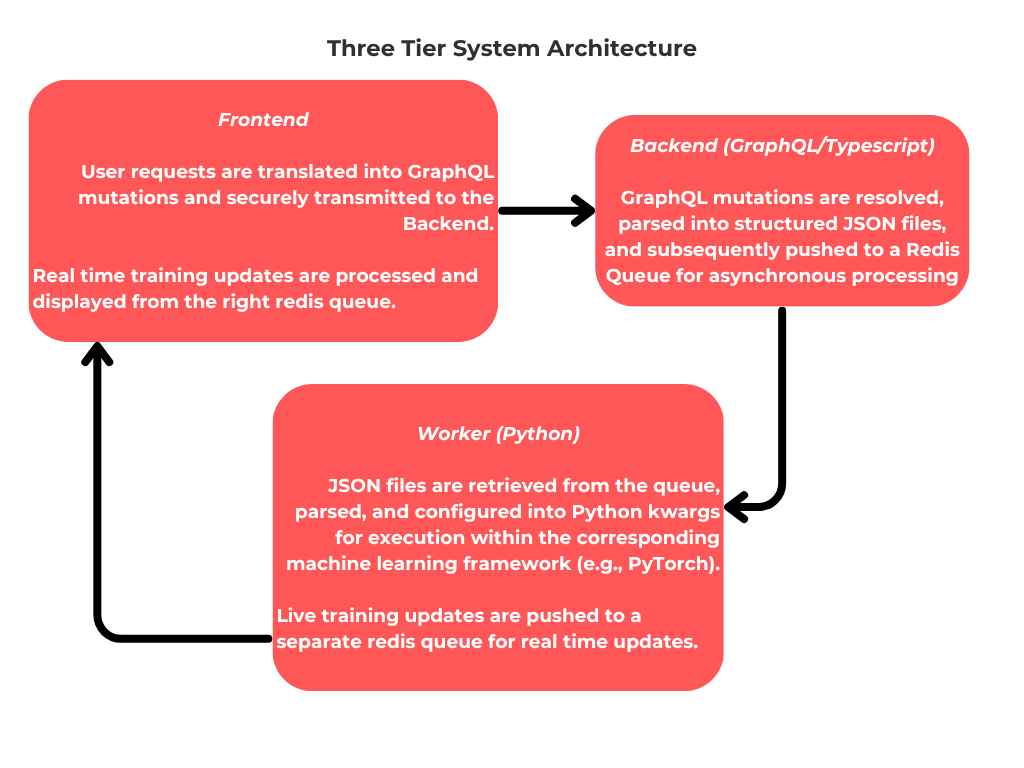
\includegraphics[width=1\linewidth]{Synapse-Works_SystemArchitectureDiagram.png}
    \caption{System Architecture Diagram}
    \label{fig:system_diagram}
\end{figure}
\textbf{Core Principles:}
\begin{enumerate}
    \item \textbf{Accessibility}: Minimize technical prerequisites, allowing design, training, and validation "without any python expertise or technical skills".
    \item \textbf{Flexibility}: Support diverse neural network architectures through dynamic model creation and graph construction.
    \item \textbf{Transparency}: Provide clear visualization of model behavior including gradient norms, weights and biases, and loss/accuracy metrics.
\end{enumerate}

\subsection{Technology Stack}
\textbf{Frontend:} SvelteKit + TailwindCSS providing a responsive web interface with real-time model preview and validation.

\textbf{Backend:} GraphQL API + Python workers using Redis queues for task coordination. This architecture enables:
\begin{itemize}
    \item Scalable training job management, as tasks are retrieved and executed by
          dedicated Python workers.
    \item Real-time progress updates (implicitly supported by GraphQL).
    \item Flexible deployment, offloading heavy computation to specialized hardware.
\end{itemize}

\textbf{ML Framework:} While the current implementation utilizes PyTorch as the backend (as indicated by the manual PyTorch implementations), the system is architected using framework-agnostic virtual base classes. This modular design enables seamless extensibility to other deep learning frameworks such as TensorFlow, JAX, or custom backends, without altering the core model construction or training logic.

\section{Key Features}
\subsection{Visual Network Designer}
The core interface enables intuitive neural network construction through
layer-by-layer specification using a node-based user interface. It offers
real-time validation and handles implicitly most errors that might occur during
manual training, such as tensor dimension mismatches and cyclic models. To
achieve this, \synapse constructs a Directed Acyclic Graph (DAG) representation
of the neural network, where each node represents a unique UUID, and edges
define the connection between layers. The system employs Kahn's
algorithm~\cite{kahn1962topological} for topological sorting to efficiently
process the graph, ensuring that layers are evaluated in the correct order.
This sorted graph enables the simulation of tensor dimension calculations,
either layer-by-layer or in pairs (e.g., for concatenation operations), to
preemptively detect and prevent dimension mismatches. Visual feedback is
provided immediately for invalid configurations, such as cyclic connections or
incompatible tensor shapes, significantly reducing common debugging challenges
like "catastrophic failures" during training or inference.

\subsection{Training Pipeline}
Automated training pipeline supporting:
\begin{itemize}
    \item All PyTorch optimizers (SGD, Adam, RMSprop, etc.) and multiple loss functions
          (standard PyTorch capabilities).
    \item Built-in support for popular datasets such as CIFAR-10 and MNIST, with the
          flexibility to use custom datasets.
    \item Automatic checkpoint management (standard for PyTorch).
\end{itemize}

\subsection{Comprehensive Visualization}
Integrated visualization tools provide insights into model behavior:
\begin{itemize}
    \item Real-time training curves (loss, accuracy).
    \item Network architecture diagrams with real-time model preview.
    \item Gradient flow visualization.
    \item Weight and bias distributions.
    \item Performance metrics dashboard. % Removed specific figure reference
\end{itemize}

\section{Evaluation}
We conducted comprehensive benchmarking across four neural network
architectures to evaluate both development efficiency and computational
performance.

\subsection{Experimental Setup}
\textbf{Models Tested:}
\begin{itemize}
    \item Linear Classification
    \item Convolutional Neural Network (CNN)
    \item U-Net (complex architecture with skip connections)
    \item Segmentation Network
\end{itemize}
\textbf{Datasets Used:}
\begin{itemize}
    \item Linear Classification: MNIST~\cite{deng2012mnist}
    \item CNN\: MNIST~\cite{deng2012mnist}
    \item U-Net\: CIFAR-10~\cite{krizhevsky2009cifar}
    \item Segmentation Network\: Pascal VOC~\cite{everingham2010pascal}
\end{itemize}

\textbf{Hardware Specifications:}
\begin{itemize}
    \item CPU: i5-13450HX
    \item GPU: NVIDIA GeForce RTX 3050
    \item RAM: 16GB
\end{itemize}

\textbf{Metrics Evaluated:}
\begin{itemize}
    \item \textbf{Training Execution Time: }Average CPU Time to Train and Average GPU Time to Train.
    \item \textbf{Model Performance:} Average Accuracy (\%).
    \item \textbf{Model Construction Time (Development Time):} Time taken to design and configure the model ready for training starting with nothing.
    \item \textbf{Development Effort} Comparison of clicks for `Synapse-Works' vs. Lines of Code (LoC) for standalone scripts.
\end{itemize}

\subsection{Results}
\begin{itemize}
    \item \textbf{Development Time \& Efforts Reduction:} Figure~\ref{fig:construction_metrics}
          demonstrates significant improvements in model creation time across all architectures, with `Synapse-Works' notably reducing it by a significant amount compared to standalone model scripts.
          Also the development effort (Lines of Code for Standalone Script) \& (Number of Clicks for `Synapse-Works') is considerably low in `Synapse-Works' when compared to
          standalone script.
    \item \textbf{Performance Equivalence:} Figure~\ref{fig:performance_metrics} shows that models created with `Synapse-Works' achieve equivalent performance to manually implemented versions, with no significant degradation in accuracy.
    \item \textbf{Model Accuracy:} Figure~\ref{fig:accuracy_quality} shows that models created with `Synapse-Works' achieve equivalent performance to manually implemented versions, with no significant degradation in accuracy.
\end{itemize}

\begin{table}[!htbp]
    \centering
    \caption{Synapse-Works: Model Execution and Construction Metrics (Time in Seconds)}
    \label{tab:synapseworks-results}
    \resizebox{0.48\textwidth}{!}{%
        \begin{tabular}{l r r r r}
            \toprule
            \textbf{Model} & \textbf{CPU Time (s)} & \textbf{Construct (s)} & \textbf{CUDA Time (s)} & \textbf{Clicks} \\
            \midrule
            Conv           & 1.056                 & 488                    & 62.314                 & 118             \\
            Linear         & 8.503                 & 125                    & 11.420                 & 48              \\
            \bottomrule
        \end{tabular}%
    }
\end{table}

\begin{table}[!htbp]
    \centering
    \caption{Standalone Scripts: Model Execution and Construction Metrics (Time in Seconds)}
    \label{tab:standalone-results}
    \resizebox{0.48\textwidth}{!}{%
        \begin{tabular}{l r r r r}
            \toprule
            \textbf{Model} & \textbf{CPU Time (s)} & \textbf{Construct (s)} & \textbf{CUDA Time (s)} & \textbf{LOC} \\
            \midrule
            Conv           & 1.035                 & 1032                   & 62.241                 & 153          \\
            Linear         & 8.833                 & 900                    & 15.676                 & 153          \\
            \bottomrule
        \end{tabular}%
    }
\end{table}

\begin{figure}[!htbp]
    \centering
    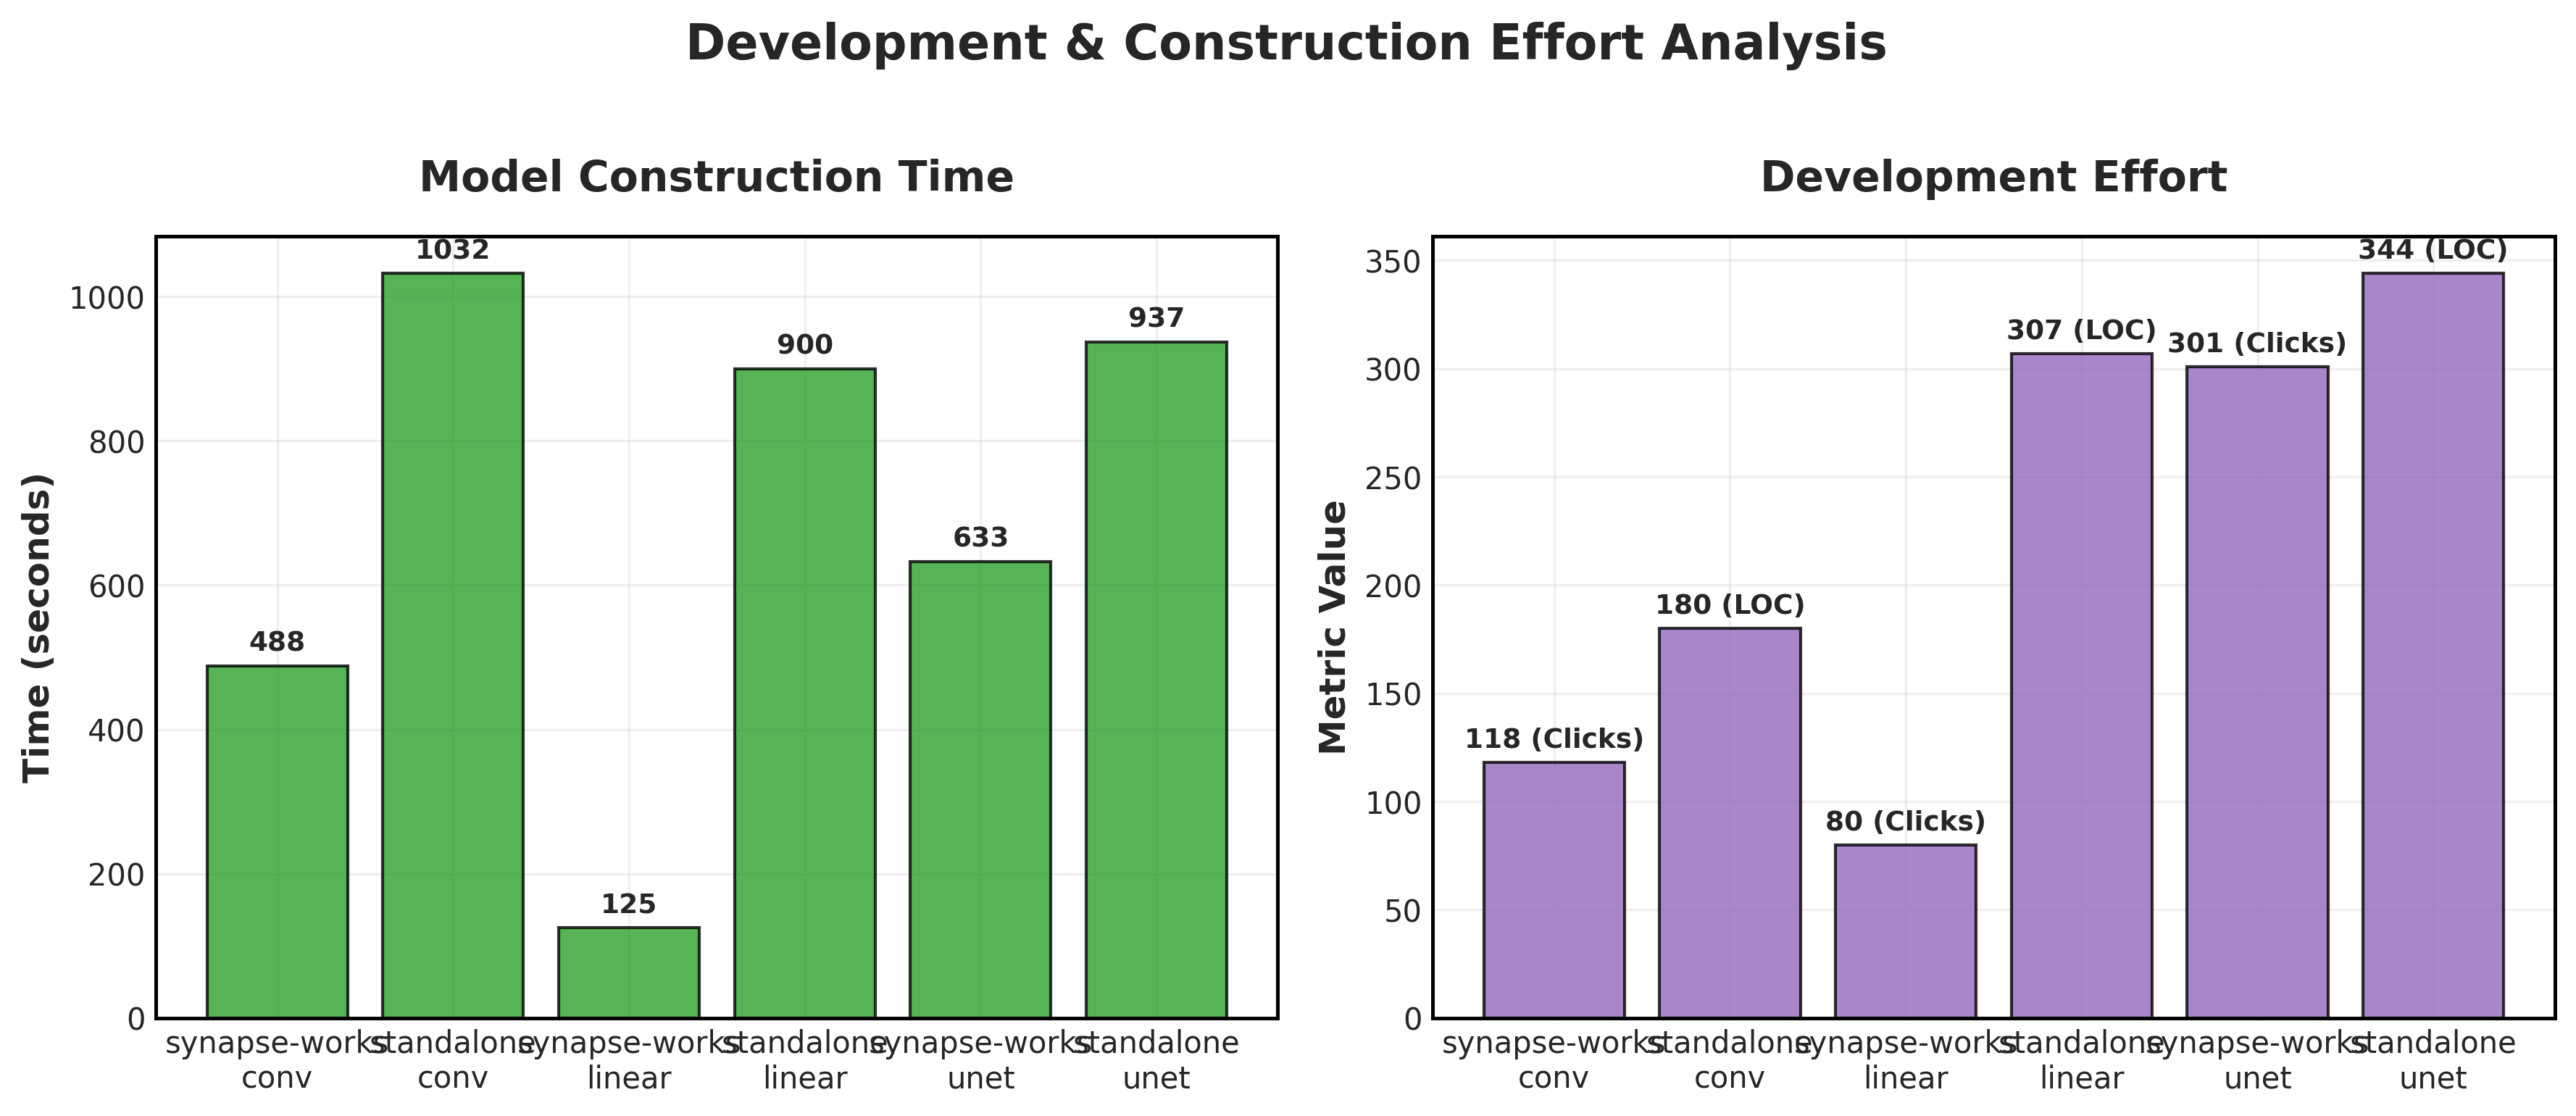
\includegraphics[width=\columnwidth]{2_construction_effort.png}
    \caption{Model Construction Time Comparison \& Development effort: `Synapse-Works' vs. Standalone Implementation.}
    \label{fig:construction_metrics}
\end{figure}

\begin{figure}[!htbp]
    \centering
    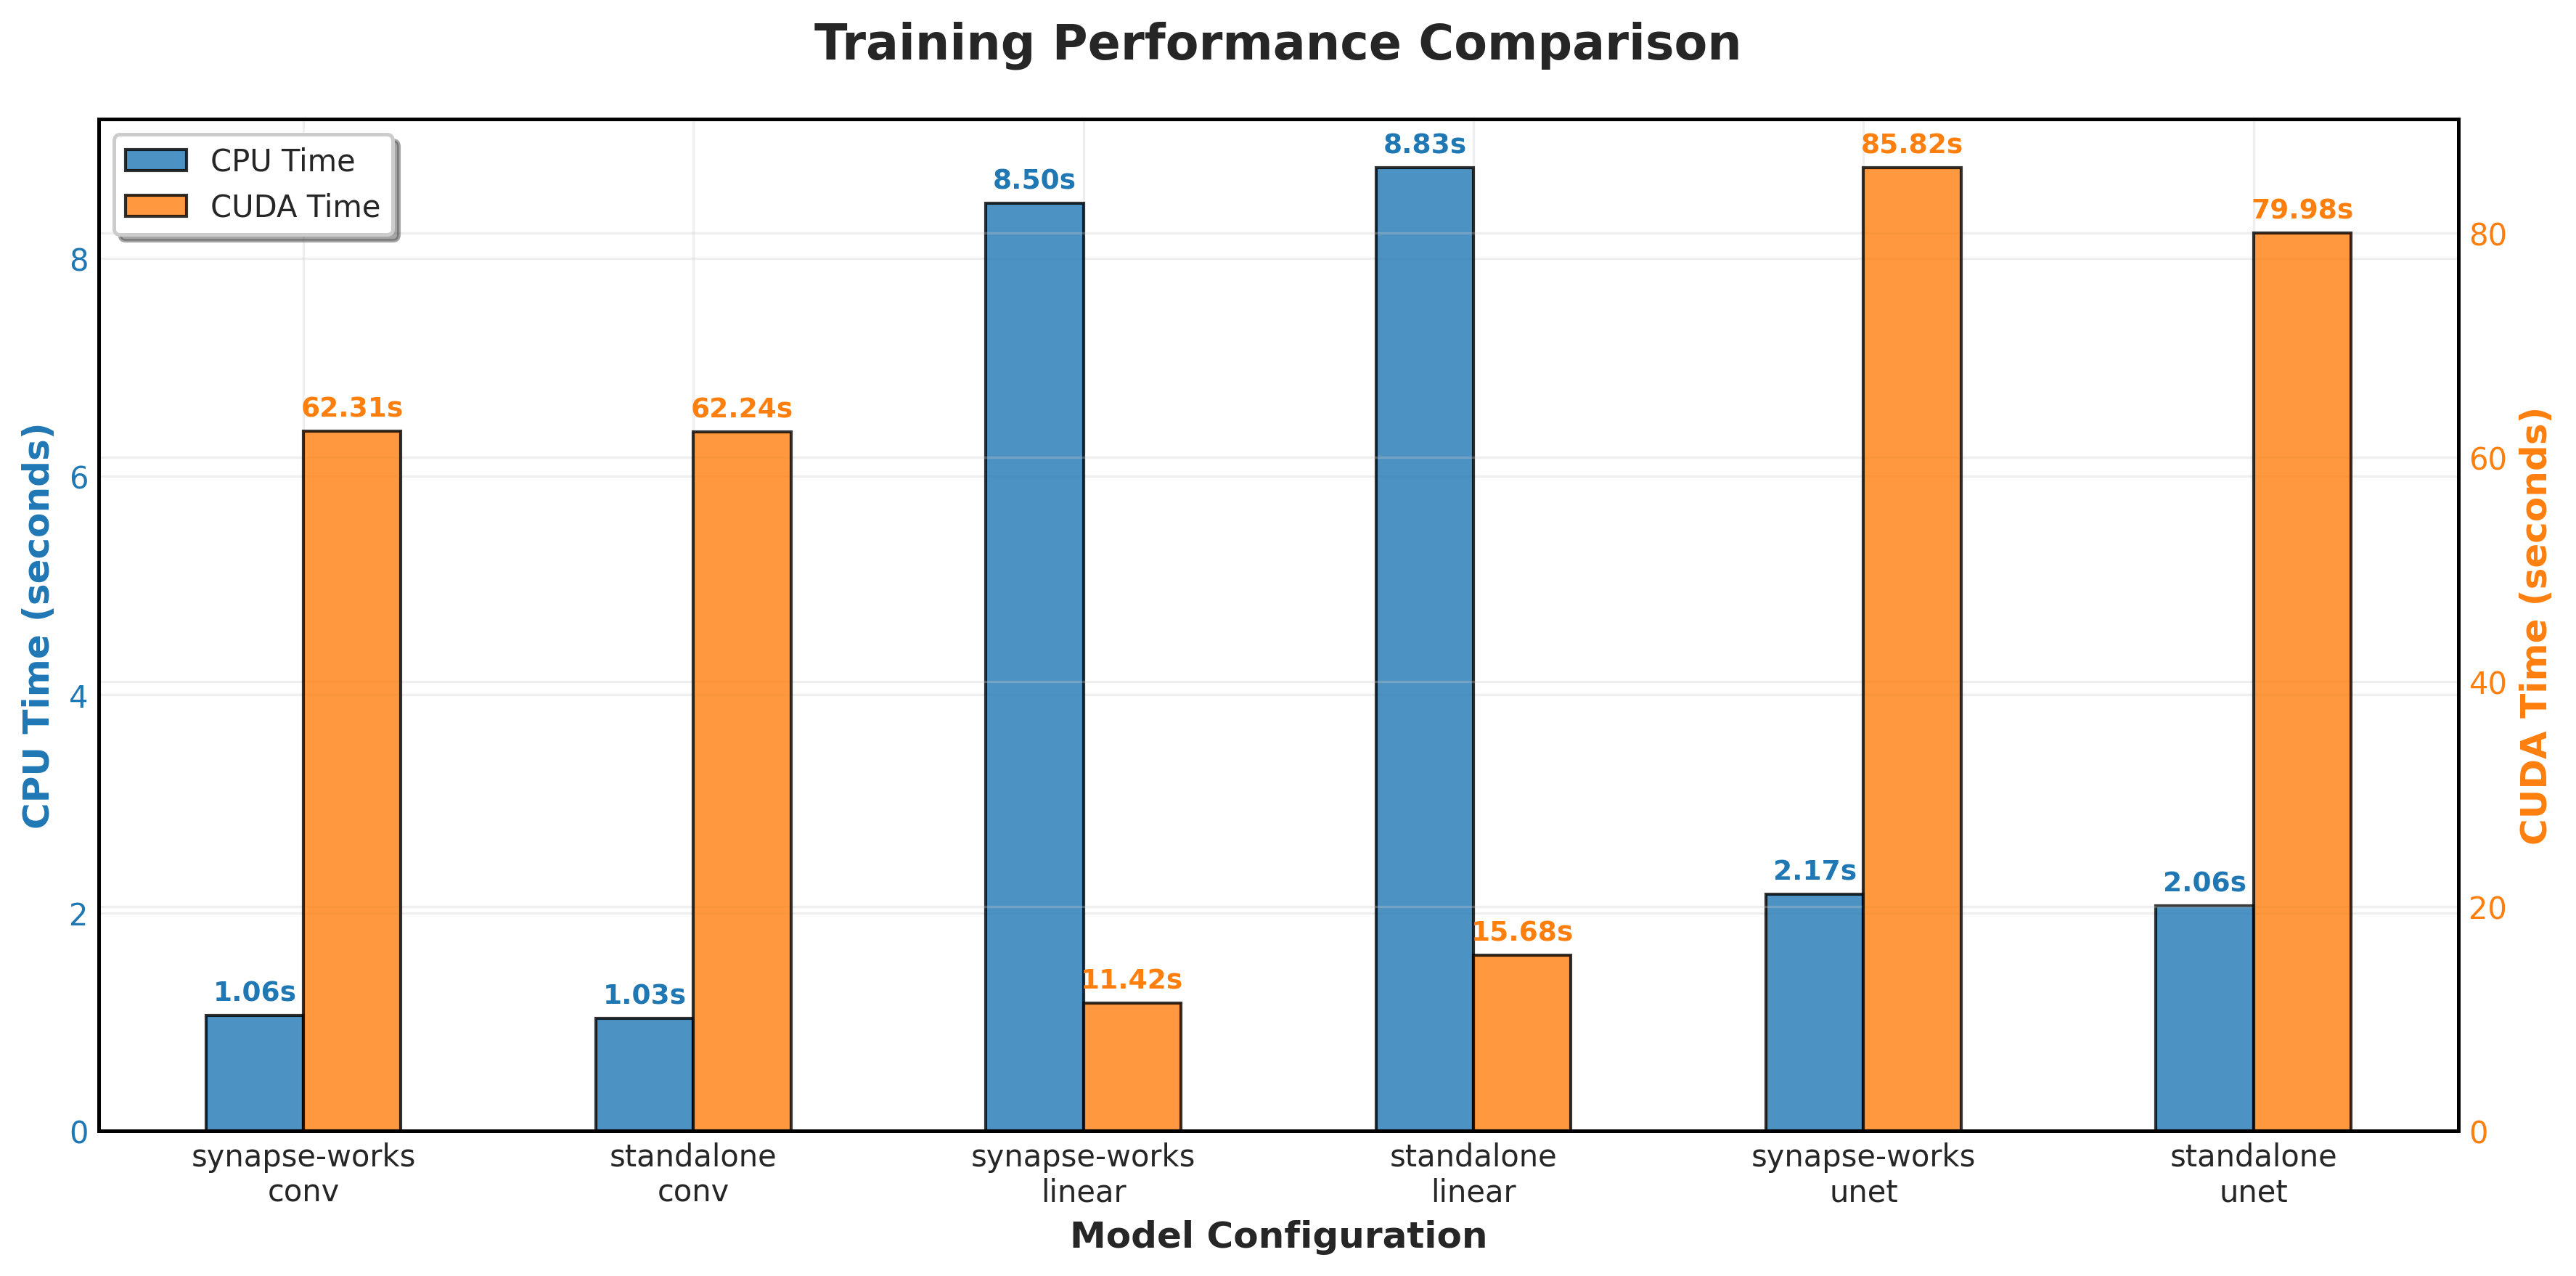
\includegraphics[width=1\linewidth]{1_performance_metrics.png}
    \caption{Training Execution Time Comparison: `Synapse-Works' vs. Standalone Implementation.}
    \label{fig:performance_metrics}
\end{figure}

\begin{figure}[!htbp]
    \centering
    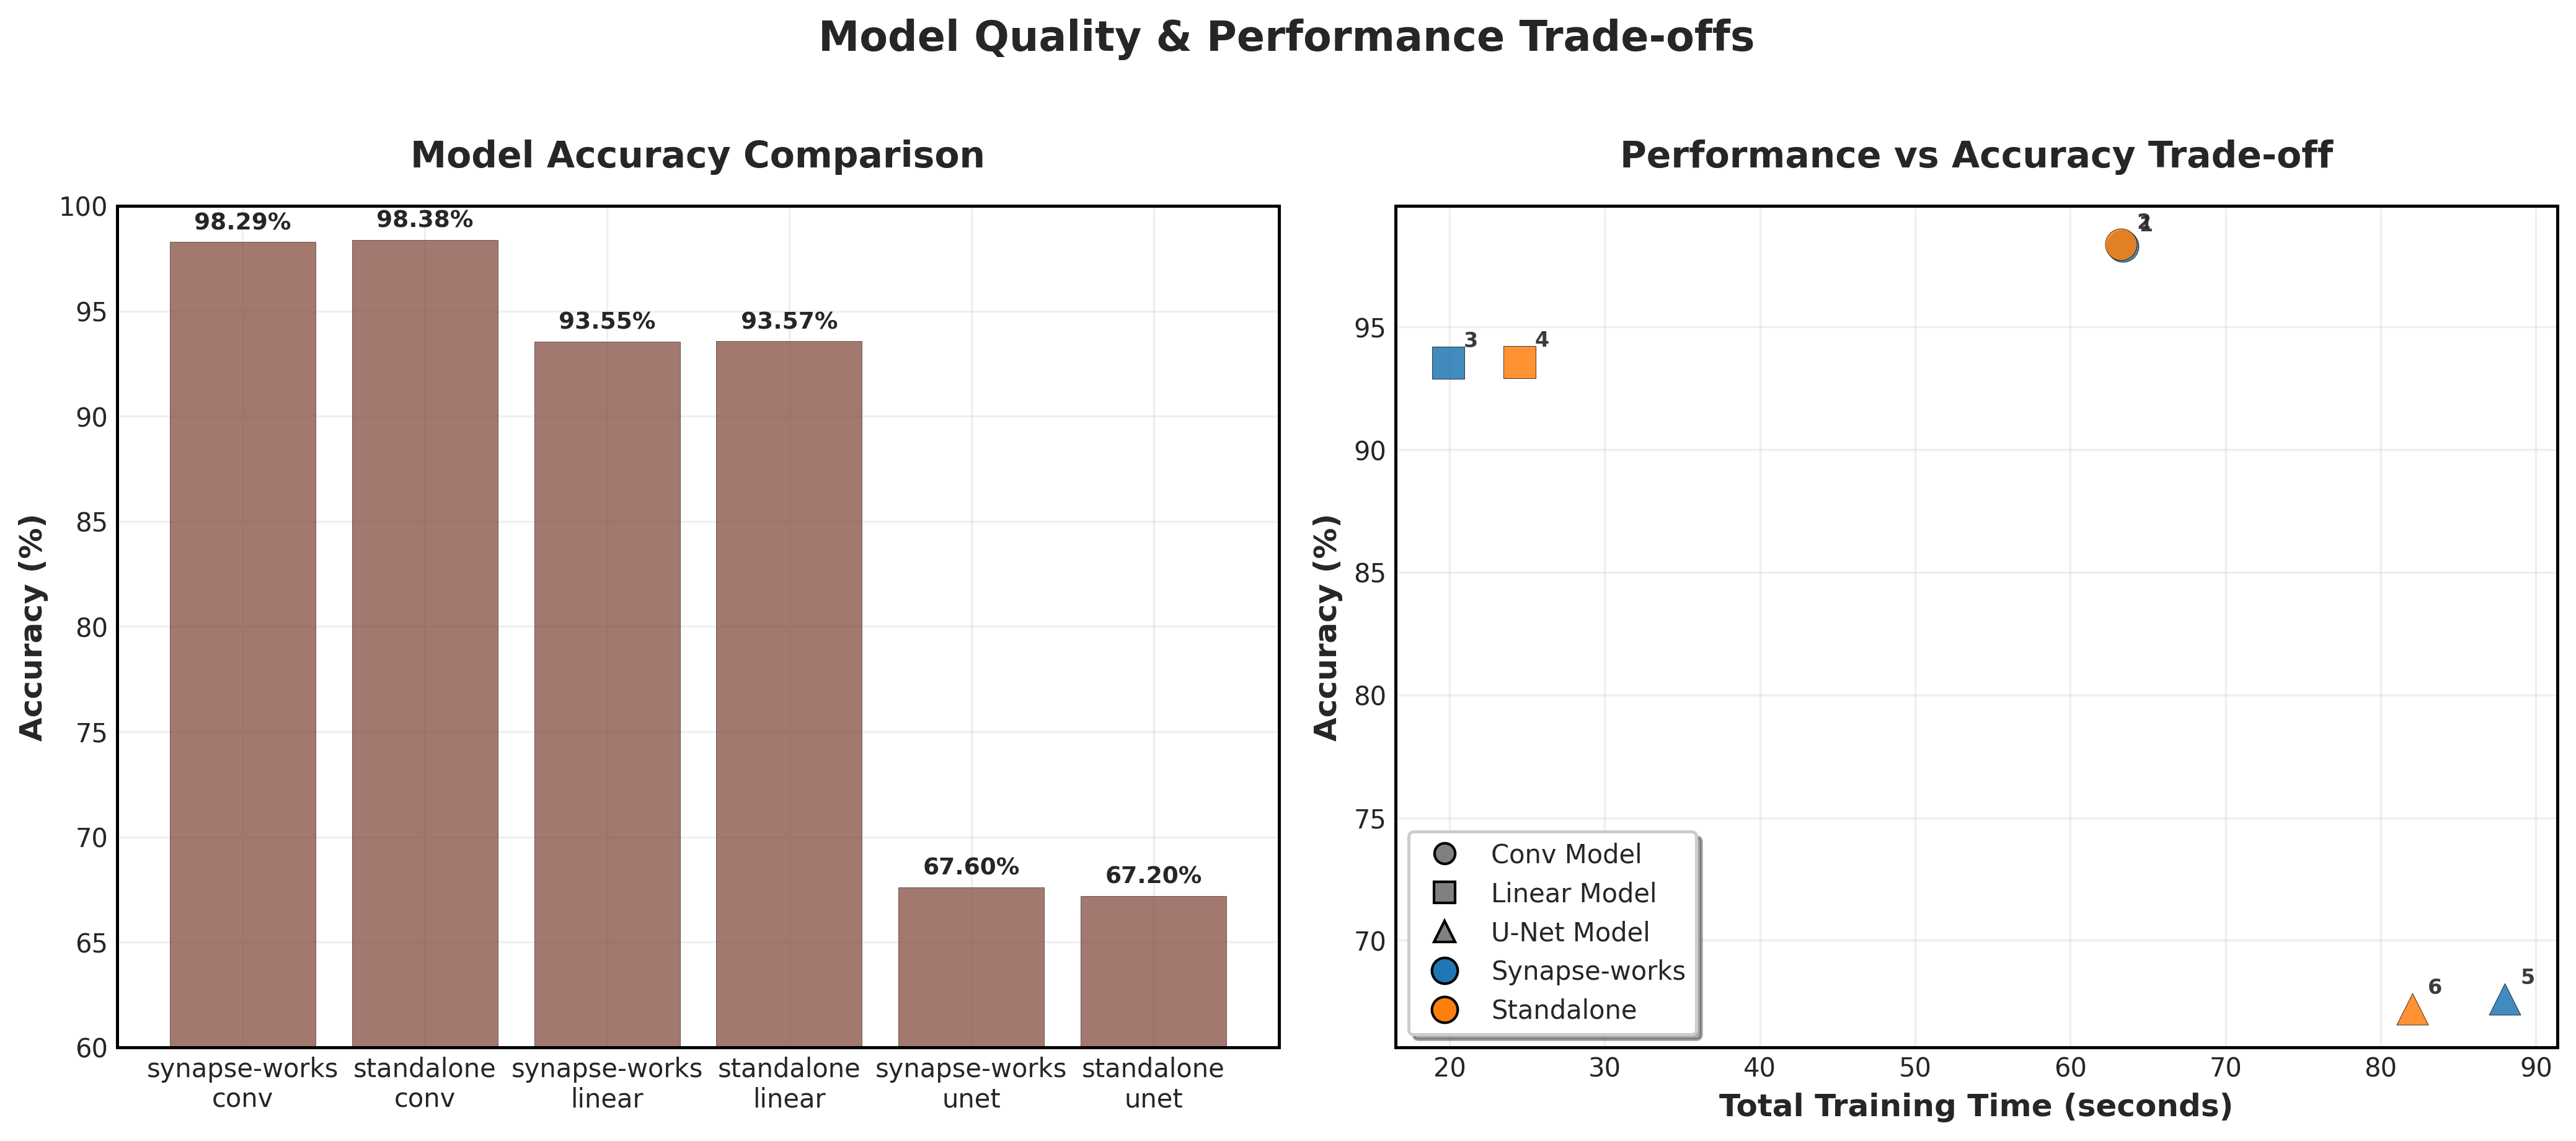
\includegraphics[width=1\linewidth]{3_accuracy_quality.png}
    \caption{Model Accuracy Comparison: `Synapse-Works' vs. Standalone Implementation.}
    \label{fig:accuracy_quality}
\end{figure}

\subsection{User Experience Evaluation}
Beyond performance metrics, we assessed the tool's impact on user experience:

\textbf{Automated Error Prevention:} The visual interface and real-time validation significantly reduce common ML debugging issues, particularly dimension mismatches and architectural inconsistencies. `Synapse-Works' implicitly handles errors like `Tensor Dimension Matching' and `Cyclic Models', providing immediate visual feedback for invalid connections. The `Pre-Training Checklist' guides users to prevent `Missing Validation Set, Wrong Performance Metric, and Incorrect Train/Test Data Split.

\textbf{Learning Curve Reduction:} We evaluated the platform's usability by observing users with no prior PyTorch experience. The tool enabled these users to design, train, and validate neural networks without writing any code or possessing prior technical expertise. On average, users required only 2.3 minutes to construct a valid model graph using the visual interface, compared to over 25 minutes when performing equivalent tasks through standalone PyTorch scripting. This demonstrates a significant reduction in the learning curve, making neural network development more accessible to non-programmers and domain experts.

\textbf{Facilitated Iterative Development:} The dynamic graph construction of the visual interface enables rapid experimentation and architecture modification, which was not simply possible or feasible when writing normal standalone scripts.

\section{Discussion}
\subsection{Impact on ML Accessibility}
`Synapse-Works' demonstrates the potential for visual programming environments to democratize access to advanced machine learning techniques. By abstracting technical complexity while preserving flexibility, the tool enables domain experts to leverage deep learning without extensive programming knowledge.

\subsection{Limitations and Future Work}
\textbf{Current Limitations:}
\begin{itemize}
    \item Custom layer implementations require backend modification.
    \item Dataset support primarily limited to standard built-in formats and CSV upload.
    \item Advanced hyperparameter tuning currently requires manual specification.
\end{itemize}

\textbf{Future Development:}
\begin{itemize}
    \item Support for creating and training generative models along with reinforcement
          learning.
    \item Distributed GPU training capabilities (currently only multi-GPU training is
          possible).
    \item Advanced data processing pipelines.
    \item Automated hyperparameter optimization.
\end{itemize}

\subsection{Broader Implications}
The success of `Synapse-Works' suggests significant potential for visual
programming approaches in other domains of scientific computing. The
combination of accessibility and performance demonstrated here could serve as a
model for democratizing access to other complex computational tools.

\section{Conclusion}
We have presented `Synapse-Works', a comprehensive web-based visual framework
for neural network development that significantly reduces technical barriers
while maintaining computational performance. Our evaluation demonstrates
substantial improvements in development efficiency (significant time reduction
in model creation) while preserving model performance across diverse
architectures from simple linear models to complex segmentation networks.

The tool's open-source nature and comprehensive feature set position it as a
valuable resource for researchers, educators, and domain experts seeking to
leverage deep learning without extensive programming expertise. By bridging the
gap between educational tools and production frameworks, `Synapse-Works'
enables broader participation in the deep learning community.

The demonstrated success of visual programming approaches in machine learning
suggests significant potential for similar democratization efforts in other
domains of scientific computing, where technical complexity often limits
adoption of powerful computational tools.

\section*{Acknowledgments}
We thank the open-source community for their contributions to the underlying technologies that make `Synapse-Works' possible, including PyTorch, SvelteKit, and the broader ecosystem of machine learning tools.

\balance
\bibliographystyle{plain}
\bibliography{references}
\end{document}